% Created 2015-01-02 Fri 15:32
\documentclass[11pt]{article}
\usepackage[utf8]{inputenc}
\usepackage[T1]{fontenc}
\usepackage{fixltx2e}
\usepackage{graphicx}
\usepackage{longtable}
\usepackage{float}
\usepackage{wrapfig}
\usepackage{rotating}
\usepackage[normalem]{ulem}
\usepackage{amsmath}
\usepackage{textcomp}
\usepackage{marvosym}
\usepackage{wasysym}
\usepackage{amssymb}
\usepackage{hyperref}
\tolerance=1000
\input /Users/strow/Tex/Templates/article_setup
\setcounter{secnumdepth}{4}
\author{L. Strow}
\date{\today}
\title{kCARTA Documentation}
\hypersetup{
  pdfkeywords={},
  pdfsubject={},
  pdfcreator={Emacs 24.4.1 (Org mode 8.2.10)}}
\begin{document}

\maketitle
\section{Introduction}
\label{sec-1}

kCARTA stands for "kCompressed Atmospheric Radiative Transfer
Algorithm." This is an infrared, "monochromatic" radiative transfer
algorithm written for a one dimensional non-scattering Earth atmosphere.

At the heart of the code are routines to uncompress an optical depth
database, computed for the US Standard Profile and for 10 temperature
offsets (-50 K, -40K, \ldots{}, +40 K, +50 K) from this profile. This makes
computing optical depths for any realistic Earth atmosphere very fast
and accurate, as the code only needs to interpolate the arbitrary
profile using this underlying temperature grid. Uncompressing the
database also rapidly yields analytic temperature jacobians.

The code was originally written in F77, and morphed to include upwelling
and downwelling clear sky radiative transfer calculations, calculations
in a scattering atmosphere, NLTE effects in the 4 um CO2 band, and
fluxes and heating rates calculations. This Matlab package encapsulates
the uncompression routines, and provides examples of how to produce
clear sky optical depths and radiative transfer calculations. The
package is tied in with UMBC kLAYERSand "RTP" packages. The former takes
a levels profile, and produces a layers averaged profile. The latter is
a .hdf based file format, and allows us to include all necessary
parameters (such as profile information, satellite and solar angles,
emissivities) into a "Radiative Transfer Protocol" file.

\section{Radiative transfer}
\label{sec-2}

For a downward looking instrument, in a clear sky, the surface term and
layer emission terms are automatically included in the radiative
transfer calculation. In addition, reflected thermal and solar terms can
also be included :

$$R(\nu) = R_{\mathrm{surface}}(\nu) + R_{\mathrm{layer\, emission}}(\nu) + 
R_{\mathrm{thermal}}(\nu) + R_{\mathrm{solar}}(\nu)$$

where the terms are the surface, layer emissions, reflected thermal and
solar respectively. The reflected thermal term is computed accurately by
determining (monochromatically) the layer to ground cumulative sum of
absorption coefficients, and then using an optimum diffusive angle based
on a parameterization of angle as a function of this cumulative sum.
This makes the inclusion of reflected thermal in the code quick and
accurate. By differentiating the radiance equation with respect to a
layer gas amount or temperature, the radiance Jacobian is obtained.
Dropping the surface and reflected thermal terms enables kCARTA to
compute the radiance measured by an upward looking instrument as well.
The radiative transfer routines include effects of curvature on angles
that deviate from nadir.

More documentation on the driver files, and on the convolution routines,
can be found in the appropriately named pdf files.

\section{Analytic Jacobians}
\label{sec-3}

Taking into account the view angle correction, if $\tau_{i}$ is the
optical depth due to gas G at layer $i$, given by
$\tau_{i} = q_{i} K_{i}/\mu{i}$ where the symbols respectively stand for
optical depth (dimensionless), gas amount (kmoles/cm2), gas absorption
(cm2/kmol) and $\cos(\mathrm{view angle})$, then the finite difference
column gas jacobian is given by the difference between the new and
unperturbed radiances $\delta r$ = $r_{new} - r_{0}$ when the gas
amounts in layers $1$ to $N$ are perturbed by a fraction $\delta$. The
(finite differences) column jacobians can be obtained from the (gas)
layer analytic jacobians using
$$\delta r = \frac{\partial r}{\partial q_1} \delta q_1 + 
           \frac{\partial r}{\partial q_2} \delta q_2 + ... + 
           \frac{\partial r}{\partial q_N} \delta q_N$$

or

$$\delta r = J_{1} \delta q_1 + J_{2} \delta q_2 + ...
               J_{N} \delta q_N$$ 

Usually we take a constant
perturbation to the column ie $q_{l} \rightarrow 
q_{1}(1 + f)$ where $f \ll 1$. Then $\delta q_{l} \rightarrow f q_{l}$
and $\delta r = f(J_{1} q_1 + J_{2} q_2 + ... + J_{N} q_N )$. For
example, for a 2 layer atmosphere the upwelling radiance (without
background thermal or solar terms)jacobian terms $J_{l}$ is

$$\begin{aligned}
r = & \epsilon B(T_{s}) exp(-q_{1} K_{1}/\mu_{1})exp(-q_{2} K_{2}/\mu_{2}) +\\
    & B(1)(1-exp(-q_{1} K_{1}/\mu_{1}))exp(-q_{2} K_{2}/\mu_{2}) + \\
    & B(2)(1-exp(-q_{2} K_{2}/\mu_{2}))\end{aligned}$$

from which the layer jacobian terms $J_{i}$ reduce to

$$\begin{aligned}
J_{1} = \frac{\partial r}{\partial q_1} = & 
 -\frac{K_1}{\mu_1}\epsilon B(T_{s})exp(-q_1 K_1/\mu_1)exp(-q_2 K_2/\mu_2) + \\
&-\frac{K_1}{\mu_1} B(1)(exp(-q_{1} K_{1}/\mu{1})exp(-q_{2} K_{2}/\mu{2})\end{aligned}$$

$$\begin{aligned}
J_{2} = \frac{\partial r}{\partial q_2} = & 
-\frac{K_2}{\mu_2}\epsilon B(T_{s})exp(-q_1 K_1/\mu_1)exp(-q_2 K_2/\mu_2) + \\
& -\frac{K_2}{\mu_2} B(1)exp(-q_{1} K_{1}/\mu{1})exp(-q_{2} K_{2}/\mu{2}) + \\
& -\frac{K_2}{\mu_2} B(2)exp(-q_{2} K_{2}/\mu{2})\end{aligned}$$

\section{kCompressed Database}
\label{sec-4}

Optical depths are computed for all molecules in the HITRAN database,
using a profile derived from the 1962 US Standard Atmosphere. These
optical depths are pre-computed using a Matlab based line by line code.

The current database spans 605 cm$^{\text{-1}}$ to 2805 cm$^{\text{-1}}$ , broken up into chunks
that are 25 cm$^{\text{-1}}$ wide. The point spacing of the current database is
0.0025 cm$^{\text{-1}}$ , which is an average over five points spaced at 0.0005 cm$^{\text{-1}}$
. One hundred pressure layers are used to generate the database, from
1100 mb down to 0.005 mb. These pressure layers are the same as those
used for the AIRS (Atmospheric InfraRed Sounder) Fast Forward Model, for
which kCARTA is the "Reference Forward Model."The thickness of the
layers is roughly 250 m close to the surface, gradually increasing to as
much as 2000m in the upper atmosphere. The 100 layers were carefully
chosen so as to keep errors at the 0.1 K level, comparable to noise
levels in contemporary sounders.

The temperatures in the spectroscopic database are computed at the
Standard Profile, as well as ten temperature offsets (in increments of
$\pm$ 10K) on either side of the Standard Profile. These optical depth
tables are compressed using a Singular Value Decomposition (SVD)
technique, to produce our kCompressed database.

The current spectroscopic compressed tables use the HITRAN98 database
for both line-parameters and cross-sections. The full and first-order
$CO_{2}$ linemixing is from refining the modeling undertaken by David
Tobin. It should be more accurate than that currently in GENLN2. in
addition, we have used the latest O2 and N2 continuum models (see
Lafferty and J.-M. Hartmann et al in Applied Optics 1996, 1997). Other
updates to spectroscopy include the "local" water lineshape as defined
by CKD.

To compute the absorption coefficients for an arbitrary profile, the
look-up tables are interpolated in temperature, and scaled in gas
absorber amount. These interpolations allow easy computation of analytic
temperature derivatives, from which we can compute temperature
Jacobians. kCARTA is not limited to these 100 AIRS pressure
levels/layers. The user can change the pressure levels scheme in
kLAYERS, and kCARTA will then also do a pressure interpolation (as long
as the new pressures span 1100 to 0.005 mb).

The speed and features of the code make it an appealing alternative to
other existing "line by line" codes such as GENLN2 and LBLRTM. The
accuracy of the database has been extensively compared to GENLN2. kCARTA
should contain the latest spectroscopy/lineshape information. The
transmittances computed by kCARTA are smooth and well behaved, which
will allow people to develop fast-forward models.

\section{GasIDs}
\label{sec-5}

The gasIDs used by kCARTA and kLAYERSfollow the HITRAN convention.
\texttt{gasids\_H2008} (and the earlier \texttt{gasids\_H92\_H2k}) in this \texttt{DOCS}
subdirectory, provide a list of gasID vs commonly used name and/or
chemical formula.

\section{Units and Definitions}
\label{sec-6}

Frequencies are in units of wavenumbers (cm$^{\text{-1}}$ ), temperatures are in
Kelvins. The gas profiles expected by kCARTA use path averages over the
layers, and are in units of $\hbox{\em molecules} {\hbox{cm}}^{-2}$.
Temperatures should be specified in \emph{kelvin}, while pressures and
partial pressures should be expressed in \emph{millibar}.

Output gas and mixed path optical depths are dimensionless (absorption
coefficient $\times$ gas amount); obviously so are transmittances.
Output radiances are in blackbody radiance units
$m^{-2} sr^{-1}/{\hbox{cm}}^{-1}$. Jacobians can be output in one of
three modes : (a) $d(r)/ds_{m}$, where $s_{m}$ is the temperature or gas
amount in layer $m$, (b) $d(r)/ds_{m} \times Z_{m}$, where $s_{m}$ is
the temperature or gas amount in layer $m$, and $Z_{m}$ is an unit
perturbation (+1 K if temperature, or +gas amount in $m^{th}$ layer) and
(c) $d(BT)/ds_{m} \times Z_{m}$, where $s_{m}$ is the temperature or gas
amount in layer $m$, and $Z_{m}$ is an unit perturbation (+1 K if
temperature, or +gas amount in $m^{th}$ layer)

\section{Installation}
\label{sec-7}

This is for the user that wants to install and use kCARTA as quickly as
possible. We purposely keep this user manual short, and ask the user to
examine the \texttt{user\_set*.m} codes in the \texttt{Test} subdirectory in orderto
understand how to use the package.

The distribution is divided into three parts :

\begin{itemize}
\item Matlab source on \href{http://github.com/strow/kcarta-matlab}{github}.

\item kCompressed Database: about 600Mb, supplied via our ftp site. We
supply two versions, big or little endian.
\end{itemize}

After cloning \texttt{kcarta-matlab.git} from github, you will find the main
directory, \texttt{PACKAGE\_UPnDOWNLOOK\_2011}, and many subdirectories
containing the source code, data files and so on.

\begin{verbatim}
drwxr-xr-x 2 sergio pi_strow    7 Mar 24 17:31 Test
drwxr-xr-x 2 sergio pi_strow    4 Mar 24 17:29 RTPFILES
drwxr-xr-x 2 sergio pi_strow   13 Mar 24 17:23 DOC
drwxr-xr-x 2 sergio pi_strow   12 Mar 24 15:24 CONVOLUTION
drwxr-xr-x 6 sergio pi_strow   26 Mar 24 04:49 VariablePressure
drwxr-xr-x 6 sergio pi_strow    9 Mar 23 12:40 private
drwxr-xr-x 3 sergio pi_strow    4 Mar 23 10:35 JACDOWN
drwxr-xr-x 6 sergio pi_strow    6 Mar 22 15:38 DATA
\end{verbatim}

\section{Overview by Source Directory}
\label{sec-8}

\subsection{Main directory}
\label{sec-8-1}

This contains the main files needed if using a pressure layering that is
the same as the AIRS 100 layers, which is generally sufficient for nadir
sounders.

Routines for uncompressing the database \texttt{kcmix*.m} and the continuum
files \texttt{cont*.m}, for doing radiative transfer \texttt{rtchunk\_Tsurf*.m} are
included here. The \texttt{\_nojac} extension to the name means the faster (non
jacobian version), while \texttt{\_jac} is the slower, jacobian version. The
main routines are \texttt{matlab\_kcarta\_downlook\_.m}.

Note: if the user wants to edit which gases he/she should be included in
the "atmosphere", then look for the line that says "edit this list to
only keep gases you DO want" in \texttt{matlab\_kcarta\_downlook\_jac.m} or
\texttt{matlab\_kcarta\_downlook\_nojac.m} or \texttt{matlab\_kcarta\_opticaldepths.m}; the
default is to add $ALL$ gases.

\begin{verbatim}
Main directory files:

auxiliary_set.m
contcalc2.m
contcalc2_S_F.m
continuum_temp_interp_weights_jac.m
continuum_temp_interp_weights.m
contjaccalc2.m
dirname.m
doload.m
find_chunks.m
initialize_extra.m
initialize_kcmix.m
kcmix2jac.m
kcmix2.m
matlab_kcarta_downlook_jac.m
matlab_kcarta_downlook_nojac.m
matlab_kcarta_opticaldepths.m
nlte.m
op_rtp_to_lbl2.m
rtchunk_Tsurf_jac.m
rtchunk_Tsurf.m
temp_interp_weights_jac.m
temp_interp_weights.m
\end{verbatim}

The existing packages is optimized for the 605 - 2830 cm$^{\text{-1}}$ spectral
range which is the range covered by AIRS, IASI, CrIS, and HIRS and AERI
instruments. However the code is flexible enough to allow optical depth
and radiance calculations in other spectral bands. Since the FWHM of
lines gets smaller (larger) as the wavenumbers get smaller (larger), the
resolution of the database must change. Each file in each spectral range
will contain 10000 points; so for example at the default 0.0025 cm$^{\text{-1}}$
resolution of the main IR default band (605-2830 cm$^{\text{-1}}$ ), the files each
span 25 cm-1 . We envisage the following :

\begin{verbatim}
kcartachunks = 00080 : 0002.5 : 00150;  prefix = '/j';
kcartachunks = 00140 : 0005.0 : 00310;  prefix = '/k';
kcartachunks = 00300 : 0010.0 : 00510;  prefix = '/p';
kcartachunks = 00500 : 0015.0 : 00605;  prefix = '/q';
kcartachunks = 00605 : 0025.0 : 02830;  prefix = '/r'; ** default **
kcartachunks = 02830 : 0025.0 : 03580;  prefix = '/s';
kcartachunks = 03550 : 0100.0 : 05650;  prefix = '/m';
kcartachunks = 05550 : 0150.0 : 08350;  prefix = '/n';
kcartachunks = 08250 : 0250.0 : 12250;  prefix = '/o';
kcartachunks = 12000 : 0500.0 : 25000;  prefix = '/v';
kcartachunks = 25000 : 1000.0 : 44000;  prefix = '/u';
\end{verbatim}

It is the responsibiliy of the user to set fA,fB in the
\texttt{user\_set\_input*} files such that they only span \textbf{one} spectral range.
For example, one run covering 605-2830 cm-1 is fine, as is another run
covering 500-605 cm-1 . But the code as written will not permit a single
run covering 500-2830 cm-1 .

\subsection{private}
\label{sec-8-2}

This subdir contains files that are called by the main routines, and
should not be modified.

\subsection{DOC}
\label{sec-8-3}

The documentation for this package

\subsection{CONVOLUTION}
\label{sec-8-4}

Convolution routines. We include generic gaussian convolvers, as well as
AIRS SRF convolvers, and IASI/CRiS convolvers. Note the files contained
in this subdir will not be supported.

\subsection{JACDOWN}
\label{sec-8-5}

This has the main driver for a downlook jacobian calculation,
\texttt{jac\_downlook.m} which calls files in the $private$ subdirectory
underneath this. One can speed up the jacobian code by eg removing the
looping over the weighting functions, or over the temperatures.

\subsection{RTPFILES}
\label{sec-8-6}

Sample rtpfiles for this package; "desert" is a downlooking case at 100
AIRS layers, while the other is an uplooking case at a different
layering scheme. In addition we provide a subdirectory with some binary
files output from the f77 code.

\subsection{DATA}
\label{sec-8-7}

Contains subdirectories with continuum, solar, NLTE and CO2 Chifunction
datafiles.

\subsection{Test}
\label{sec-8-8}

Examples of two driverfiles, one which computes optical depths (based on
a list the user supplies), and the other which computes radiances (and
jacobians if asked). The user should carefully examine these files, as
they provide a working outline of how to use this package.

Basically, the user is allowed to set the following parameters : which
HITRAN version to use, start/stop wavenumbers for the calculations,
whether or not to do Jacobians, what output units for the Jacobians,
what CKD version, and name of input rtp file.

\begin{verbatim}
user_set_input_downlook.m        parameters driving dokcarta_downlook.m
user_set_input_opticaldepths.m   parameters driving dokcarta_opticaldepths.m
\end{verbatim}

The user needs to supply paths to where the solar files, continuum
files, nlte files, klayers executables, optical depth database and
reference profiles are; this is controlled via $user_set_dirs.m$

\begin{verbatim}
user_set_dirs.m                  set up the paths to directories
\end{verbatim}

Finally the user can commence the computation, calling one or the other
of the routines named below (which call relevant files from above).

\begin{verbatim}
dokcarta_downlook.m              compute RT
dokcarta_opticaldepths.m         compute optical depths
\end{verbatim}

This subdir also includes two matlab files, containing radiances output
using H2004 and H2008.

\subsection{VariablePressure}
\label{sec-8-9}

This contains the main files a user should need for a pressure layering
different than the AIRS 100 layers. This makes the code(s) slower. The
structure and content of the directories is the same as before $viz$

\begin{verbatim}
drwxr-xr-x 2 sergio pi_strow    10 Mar 24 04:49 Test
drwxr-xr-x 6 sergio pi_strow     8 Mar 23 11:58 private
drwxr-xr-x 3 sergio pi_strow     4 Mar 23 10:36 JACUP_VarPress
drwxr-xr-x 3 sergio pi_strow     4 Mar 23 10:35 JACDOWN_VarPress
\end{verbatim}

$Test$ has \texttt{dokcarta\_downlook.m}, \texttt{dokcarta\_uplook.m} (very similar to
the "downlook" case) and \texttt{dokcarta\_opticaldepths.m.}\\

\texttt{JADOWN\_VarPress} has jacobian routines for downlooking instruments\\

\texttt{JACUP\_VarPress} has jacobian routines for uplooking instruments\\

\section{Comparisons against f77 and our code}
\label{sec-9}

We have tested this code against the f77 kCARTA code and across the IR
bands, have errors less than 0.05 K in brightness temperature. The
speeds are also very similar (roughly about 60 seconds on a 2.6 GHz
processor for a full radiative transfer calculation).

The \texttt{Test} directory contains \texttt{matlab\_test\_desert\_0725\_2004.mat} which
is a radiance computation coming from running the \texttt{dokcarta\_downlook.m}
in that directory.

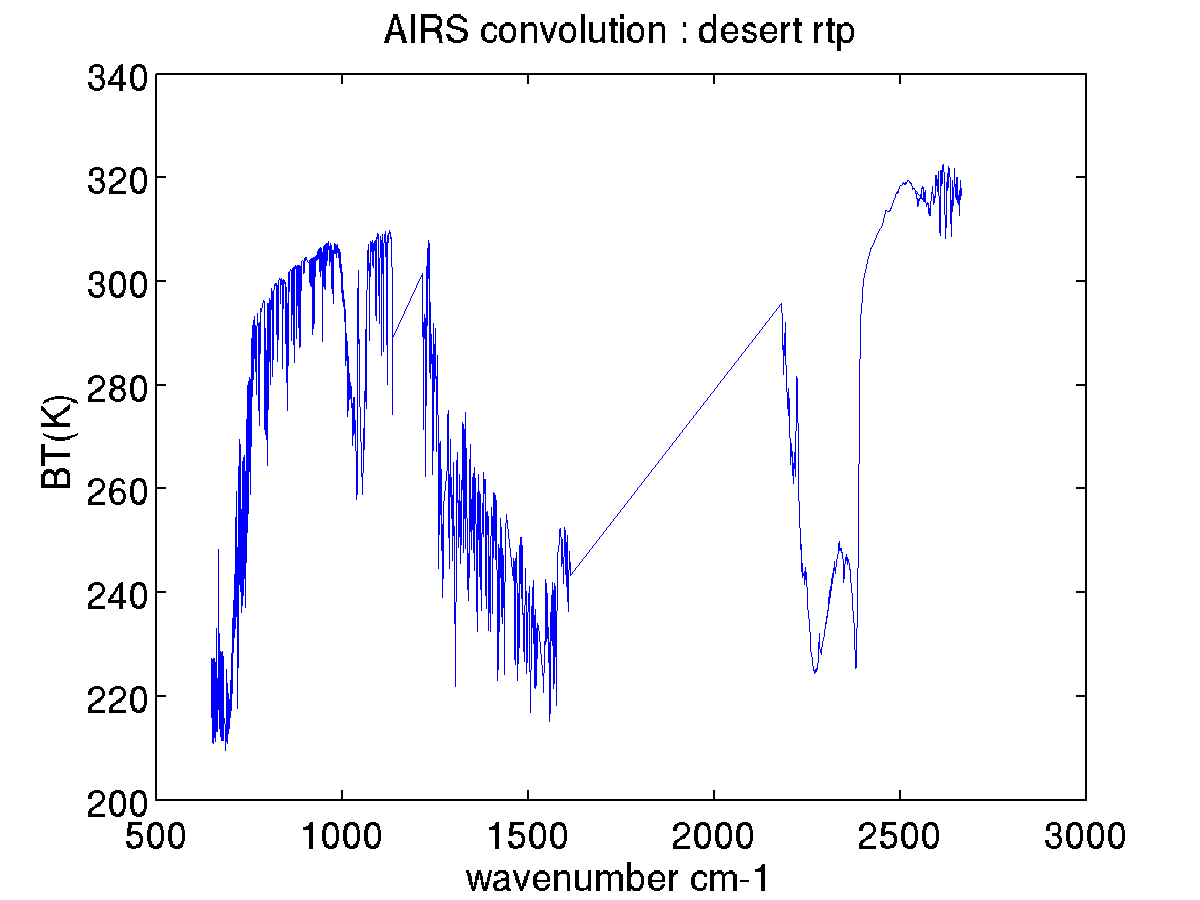
\includegraphics[width=.9\linewidth]{./desert_rtp.png}
% Emacs 24.4.1 (Org mode 8.2.10)
\end{document}